\documentclass{beamer}
\usetheme{CambridgeUS}



\usepackage{enumitem}
\usepackage{tfrupee}
\usepackage{amsmath}
\usepackage{amssymb}
\usepackage{gensymb}
\usepackage{graphicx}
\usepackage{txfonts}

\def\inputGnumericTable{}

\usepackage[latin1]{inputenc}                                 
\usepackage{color}                                            
\usepackage{array}                                            
\usepackage{longtable}                                        
\usepackage{calc}                                             
\usepackage{multirow}                                         
\usepackage{hhline}                                           
\usepackage{ifthen}
\usepackage{caption} 
\captionsetup[table]{skip=3pt}  
\providecommand{\pr}[1]{\ensuremath{\Pr\left(#1\right)}}
\providecommand{\cbrak}[1]{\ensuremath{\left\{#1\right\}}}
\renewcommand{\thefigure}{\arabic{table}}
\renewcommand{\thetable}{\arabic{table}}                                     

\title{AI1110 \\ Assignment 5}
\author{Sai Pradeep \\ AI21BTECH11013}
\date{\today}


\begin{document}
	% The title page
	\begin{frame}
		\titlepage
	\end{frame}
	% The table of contents
	\begin{frame}{Outline}
		\tableofcontents
	\end{frame}
	
	% The question
	\section{Question}
	\begin{frame}{EXAMPLE 4.25}
Q:-	 We now assume that $p$ = 0.6 and we wish to find $n$ such that the probability that k
   is between $0.59n$ and $0.61n$ is at least 0.98\\
   \end{frame}
	
	% The solution
	\section{Solution}
	\begin{frame}{Solution}
In this case. p = 0.6, q = 0.4 \\
\begin{align}
\pr{0.59n \leq k \leq 0.61n} \approx G(\dfrac{0.61 \times n- 0.6 \times n}{\sqrt{0.4\times 0.6 \times n}})-G(\dfrac{0.59 \times n- 0.6 \times n}{\sqrt{0.4\times 0.6 \times n}})
\end{align}
\begin{align}
G(x) = \int_{-\infty}^x \dfrac{e^{\dfrac{-y^2}{2}}}{\sqrt{2 \times \pi }}dy
\end{align}
\begin{align}
G(-x)=1-G(x) 
\end{align}
\begin{align}
\pr{0.59n \leq k \ 0.61n} \approx G(\dfrac{0.01 \times n}{\sqrt{0.24 \times n}})+G(\dfrac{-0.01 \times n}{\sqrt{0.24 \times n}})
\end{align}
\end{frame}
\begin{frame}{Computation}
\begin{align}
\pr{0.59n \leq k \leq 0.61n} \approx 2 \times G(\dfrac{0.01 \times n}{\sqrt{0.24 \times n}})-1 
\end{align}
Hence,
\begin{align}
 2 \times G(\dfrac{0.01 \times n}{\sqrt{0.24 \times n}})-1 \geq 0.98  \\
G(\dfrac{0.01 \times n}{\sqrt{0.24 \times n}}) \geq 0.99  \\
 \dfrac{0.01 \times n}{\sqrt{0.24 \times n}} \geq 2.35\\
0.24 \times n \geq  (\dfrac{2.35}{0.01})^2
\end{align}
   Hence, n \textgreater 13254
\end{frame}
\begin{frame}{Conclusion}
The value of n such that the probability that k is between 0.59n and 0.61n is at least 0.98 is atleast 13254.
\end{frame}
\section{Graphs}
\begin{frame}{G(x)}
\begin{figure}[htb!]
    \centering
    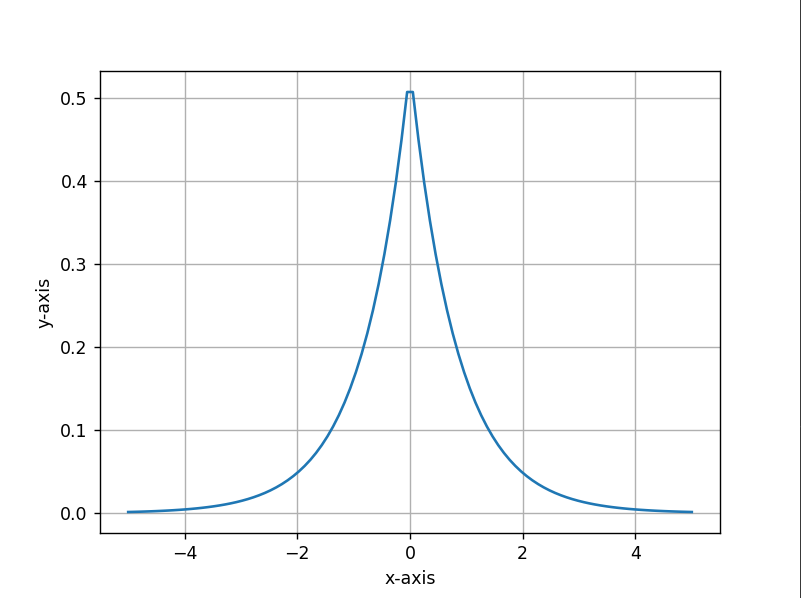
\includegraphics[width=8cm]{figures/fig1.png}
    \caption{G(x) graph}
    \label{fig:my_label}
\end{figure}
    
\end{frame}
\section{Python Output}
\begin{frame}{python output}
\begin{figure}[htb!]
 
     \centering 
     
     
     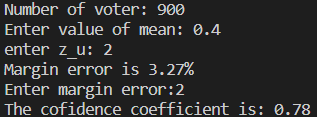
\includegraphics[width=12cm]{figures/python_output.png}
    \caption{output of python code}
    \label{fig:2}
\end{figure}
    
\end{frame}
\end{document}
 
